\chapter{Configuration Layout}
\label{ch:configuration_layout}
%\todo[inline]{From Project Guide: \\The configuration / layout shows the physical appearance of the product or system. It is mainly a set of sketches and drawings illustrating the internal and external layout with a short textual explanation.\\ The layout contains also a block diagram identifying the electronic units carried on-board.\\ A first version is presented in the Mid Term Report, generally for all design options involved in the concept selection, concentrating on those aspects that are essential to provide the trade-off.\\ The final, more detailed, version of the final design is included in the Final Report. }
This chapter outlines the details of the external and internal configuration of HUGO. \autoref{sec:external_configuration} showcases sketches of external geometry for each of the configurations considered in this design phase. Details regarding the internal components and their functions, along with a brief description of the electronic units carried on-board, are provided in \autoref{sec:internal_configuration}.
This section is not included into the trade-off process of the configurations because the internal components are the same for all designs, and layouts are similar to each other. It will serve as an analysis backbone for the final internal design, identifying necessary subsystems and their contributions. The final internal layout will be created in the next stage of the project realisation.

\section{External Configuration}
\label{sec:external_configuration}
The final design of the plane will have an external configuration that is optimised for the test section of the flight. It has a minimum number of outer ports, focusing on a smooth exterior to prevent as much as possible flow separation. 

Regardless of the smooth surface criteria, HUGO still has some outside ports, such as a pitot static tube placed under the nose cone, away from disturbed flow, the lidar port that will slightly protrude outside to scan the surrounding atmosphere, antennas for transmitting and receiving as well as the outside lights for visibility. 

Other outer characteristics include the doors for the internal components, placed in top of the fuselage, doors for the landing gear, both nose and main, camera ports and the fuel port. A sketch of the external configuration can be found in \autoref{fig:hug-cfg-303-external}.

As per calculations in \autoref{ch:engineering_design},
the aircraft requires a wingspan of 2.667 m at the maximum aspect ratio of 27. This should not cause issues with transporting the aircraft, as per van dimensions from the Baseline Report \footref{url:baseline_report}.

\begin{figure}[H]
    \centering
    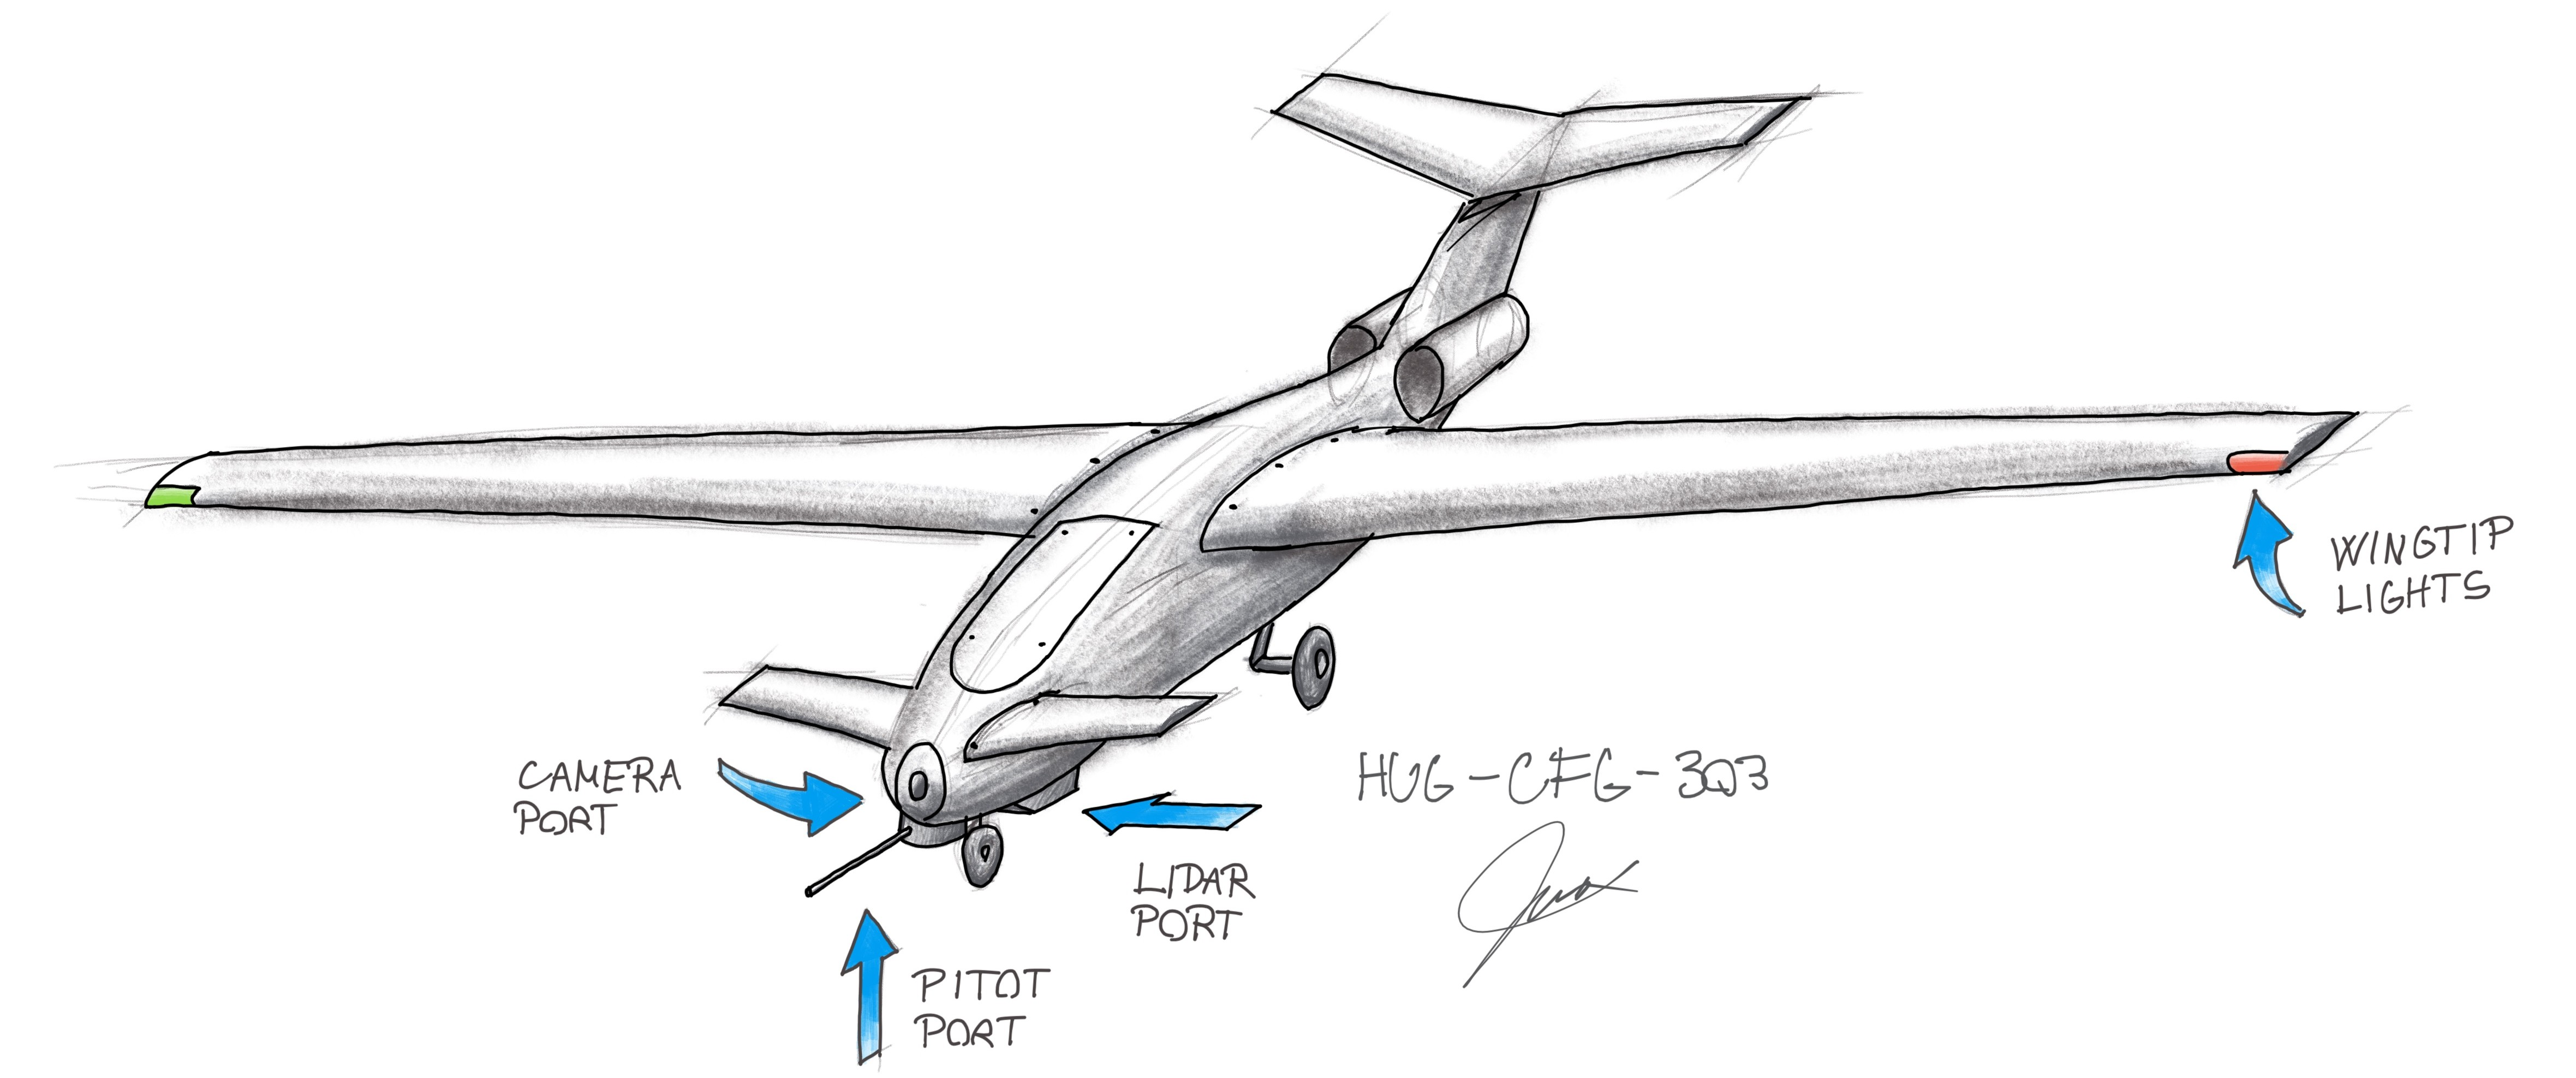
\includegraphics[width=\linewidth]{figures/Sketches/HUG-CFG-303 External Config.jpg}
    \caption{HUG-CFG-303 external configuration sketch}
    \label{fig:hug-cfg-303-external}
\end{figure}




% Include in the sketch the following:
% - pitot tube
% - liedar port
% - radar antenna
% - door for internal component
% - fuel port
% - landing gear port
% - outside lights
% - camera ports




\section{Internal Configuration}
\label{sec:internal_configuration}
This section evaluates a possible internal configuration of HUGO, mapping the layout of the electronic system, propulsion system and fuel system, along with the possible sensors to measure the aero-elastic effects during the 0.75 Mach manoeuvre.
\subsection{Electronic System}
\label{subsec:on-board_electronic_units}
Along the payload, the fuselage will house the electronic system, including the sensors and supply the payload. The engine requires an outside source of power for the start-up procedure, as such, the battery will provide the additional power needed. The margin left from the battery will power the payload, and other secondary subsystems.

A list of components included in the electronic system of HUGO can be seen in \autoref{tab:electronic_system} . For the internal configuration of HUGO, the dimensions and weight of each electronic component need to be catalogued, and in the next stage of the project, a detailed power system analysis can be conducted. For now, the numbers in \autoref{tab:electronic_system} represent a first-order approximation to enable calculation of dynamic stability and C.G. properties of the UAV. The components can be found in the project repository on GitHub \footnote{\href{https://github.com/Teo-Cokonaj/DSE-28/blob/main/docs/excel-files/Electronic\%20Components.xlsx}{Electronic Component List} (accessed on 26.05.2026)}.

For the purpose of this application, autopilot VECTOR-600 \footnote{\href{https://www.uavnavigation.com/products/autopilots/vector-600}{Vector-600} (accessed on 13.05.2026)} was chosen as it incorporates many of the basic air sensors needed to conduct the flight. Working along a flight companion, preferably made by the same company for compatibility, the system has the capability to collect the sensor data, store it, use it for flight calculations and ultimately transmit it back to the base of operations. Additionally, this autopilot has been qualified by the industry, being tested against vibrations and crash loads. It incorporates: Dual Inertial Measurement Unit (IMU), redundant inertial sensing for altitude, magnetometer, gyroscope, inertial magnetometer, altimeter, airspeed sensor, Global Navigation Satellite System (GNSS) receiver for gps signal. One limitation of this system is the maximum air speed calculator, which can only reach speeds of 450 kts, while HUGO can fly at a maximum speed of 500 kts, as such an additional speed sensor is needed. Alongside the autopilot, the design team has decided to include additional data sources such as: pitot static tube, radar system, temperature sensors, humidity sensors, cameras (one for piloting and 2 more for the view of the fuselage), and an angle of attack sensor. Storage of the data for further processing is done on a SATA SSD, with a capacity of 1TB, as it is robust and will offer enough storage space for a 30-minute flight.

\begin{table}[H]
    \centering
    \caption{Electronic system components and approximate weight and volumes}
    \begin{tabular}{|c|c|c|}
        \hline
         \textbf{Component} & \textbf{Weight [g]} & \textbf{Dimensions [mm]}  \\
         \hline\hline
         Battery  &4000&  206 x 124.3 x 70.5 \\
         \hline
         Wires &0.33 kg/1000 ft& - \\\hline
         Rotary actuators (x10) & 19 & 28.4 x 38.0 x 13.3\\\hline
         Linear actuators (control surfaces and landing gear) x 5 &200& 22.6 x 30.4 x 150 \\\hline
         Flight Controller/Autopilot & 180 & 45.0 x 68.0 x 74.5\\\hline
         Flight companion &160 & 45.0 x 68.0 x 74.5 \\ \hline
         SATA SSD & 50 & 64.5 x 42 \\ \hline
         ADS-B Transceiver and FLARM Receiver system & 120 & 57 x 82 x 30 \\ \hline
         Electric switch &-&-\\\hline
         Lights (x4)& - & - \\\hline
         Power distribution system \tablefootnote{\href{https://www.orionbms.com/downloads/documents/orionjr2_specifications.pdf}{Lithium Ion Battery Management System} (accessed on 18.05.2026)} & 250 & 180 x 100 x 40 \\\hline
          
    \end{tabular}
    \label{tab:electronic_system}
\end{table}


The electronic system is complemented by a multitude of sensors present inside and on the wings and tail to study the aeroelastic behaviour of structures. A list of sensors that have been considered for the aeroelastic analysis can be found in \autoref{wing_structural_sensors}.

The nose cone will house a weather radar and a liedar sensor specific for atmospheric measurements, giving HUGO weather prediction capabilities, aiding in measuring the atmospheric parameters.

\begin{longtable}{|p{0.32\linewidth}|p{0.60\linewidth}|}
\caption{Candidate sensors for aeroelastic response measurements}
\label{wing_structural_sensors} \\

\hline
\textbf{Sensor} & \textbf{Use on wing} \\
\hline\hline
\endfirsthead

\hline\hline
\textbf{Sensor} & \textbf{Use on wing} \\
\hline\hline
\endhead

\hline
\multicolumn{2}{r}{\textit{Continued on next page}} \\
\endfoot

\hline
\endlastfoot

Foil strain gauges 
& Estimate wing-root bending moment, spar loads, and local stress through calibrated strain measurements. \\
\hline

Strain gauge rosettes 
& Measure torsion, shear, and principal strain near spars, wing roots, cut-outs, and complex load paths. \\
\hline

Wheatstone bridge strain gauge circuits 
& Convert strain measurements into bending moment, shear force, or torsional load through calibration. \\
\hline

Fibre Bragg Grating sensors 
& Measure spanwise strain along the spar and support distributed load estimation and wing deformation reconstruction. \\
\hline

FBG-based shape sensing 
& Reconstruct wing bending and twist from distributed strain measurements along the wing structure. \\
\hline

Linear Variable Differential Transformers (LVDTs)
& Measure static wing deflection during structural tests and calibration loading cases. \\
\hline

String potentiometers / draw-wire sensors 
& Measure wing-tip deflection during ground tests or structural calibration tests. \\
\hline

Inclinometers / tilt sensors 
& Support wing twist or slope reconstruction when placed at selected spanwise locations. \\
\hline

Small IMUs along the wing 
& Estimate dynamic wing motion, bending response, and torsional behaviour during flight. \\
\hline

Accelerometers 
& Measure modal response, gust response, flutter behaviour, and aeroelastic vibration. \\
\hline

MEMS IMUs 
& Measure wing-tip motion, torsional response, and flexible-body dynamics during flight. \\
\hline

Piezoelectric patches 
& Monitor flutter, vibration, and dynamic aeroelastic response; can also support active aeroelastic control concepts. \\
\hline

Acoustic emission sensors 
& Detect crack initiation, delamination, or local structural damage events for structural health monitoring. \\
\hline

Control-surface position sensors 
& Correlate structural response with commanded control input and real control-surface motion. \\
\hline

Actuator current sensors 
& Provide an indirect indication of hinge moment, actuator loading, binding, or overload during manoeuvres. \\
\hline

Lidar Sensor
& Provides 3D measurements and real-time view of the wing through a laser-based measurement system. \\
\hline

\end{longtable}


%\subsection{On-board Electronic Units}

\subsection{Fuel and propulsion system}
\label{subsec:fuel_systems}
Systems related to propulsion, including the turbojet engine, fuel tanks, fuel management, and distribution systems are included in this category. The propulsion system is integrated into the fuselage group to allow for wing versatility, provide clean airflow over the wing and prevent aerodynamic interference of the engine with the wings. This has been determined for all of the configurations in \autoref{ch:trade-off}.

The initially selected VULCAN engine is in an early development stage, and the figures regarding its overall propulsive efficiency are uncertain. Furthermore, small turbojet engines on the market can be easily integrated due to their known characteristics and availability of the supporting subsystems. Therefore, based on the approximate thrust requirement found in \autoref{sec:matching_diagram}, a pair of Jetcat P100-RX-BL engines \footnote{\href{https://www.jetcat.de/de/productdetails/produkte/jetcat/produkte/RC\%20ENGINES/Engines/p100_rx-bl}{Jetcat P100-RX-BL engine} (accessed on 19.05.2026)} are selected as the candidate engines for HUGO and are used as a reference component in \autoref{tab:prop_system}.


\begin{table}[H]
    \centering
    \caption{Propulsion system components and approximate weight and volumes}
    \begin{tabular}{|c|c|c|}
        \hline
        \textbf{Component} & \textbf{Weight [g]} & \textbf{Dimensions [mm]}  \\
        \hline\hline
        Engine: JetCat P100-RX-BL (X2) & 1080 & 97 (diameter) x 241 (length)\\
        \hline
        ECU (V10.0) (X2) & 26 & 55 x 36 x 18 (length x width x height) \\
        \hline
        Fuel tank & 0.57 & N/A (fuel bag, 3 gal capacity) \tablefootnote{\href{https://giantloopmoto.com/products/armadillo-bag?variant=61789625712970\#features}{Armadillo Bag} (accessed on 22.05.2026)}\\
        \hline
        Fuel pump (Bus-system BL) (X2)& 110 & 31.5 (diameter) x 77 (length)\\
        \hline
        Fuel filter (Standard Inline) (X2)& 15 & 20 (diameter) x 45 (length) \\
        \hline
        Fuel hoses & 170 & 8 x 4 x 2000 (outer x inner diameter x length) \\
        \hline
    \end{tabular}
    \label{tab:prop_system}
\end{table}

The turbojet engine needs additional components to become operational. An Engine Control Unit (ECU) is necessary to control combustion.The fuel system consists of the fuel pump, fuel filter, shut-off valve and fuel distribution hoses \footnote {\href{https://www.jetcat.de/en/products/produkte/jetcat/kategorien/Zubehoer}{JetCat fuel system accessories} (accessed on 18.5.2026)}. An overview of the propulsion system components is presented in \autoref{tab:prop_system} and a simple diagram of the subsystem is shown in \autoref{fig:prop_diagram}. The weight and dimensions of the power distribution system were estimated based on a universal Battery Management System (BMS) \footnote{\href{https://www.orionbms.com/downloads/documents/orionjr2_specifications.pdf}{Lithium Ion Battery Management
System} (accessed on 18.5.2026)}. Furthermore, 2m of Polytetrafluoroethylene (PTFE) tube for fuel distribution is added and a 3 gal fuel bag will be used for fuel storage \footnote{\href{https://ptfetubeshop.com/en/product/ptfe-tube-4-mm-x-8-mm/?srsltid=AfmBOopcWd4OwpWvWxhcXm5ZaT8P1H2EP4Aw9Il2Rezb7qgHZba8-M9b}{PTFE tube 4 mm x 8 mm} (accessed on 19.5.2026)}. This corresponds to the fuel mass estimated in \autoref{sec:trade-off_matrix}.


\begin{figure}[H]
    \centering
    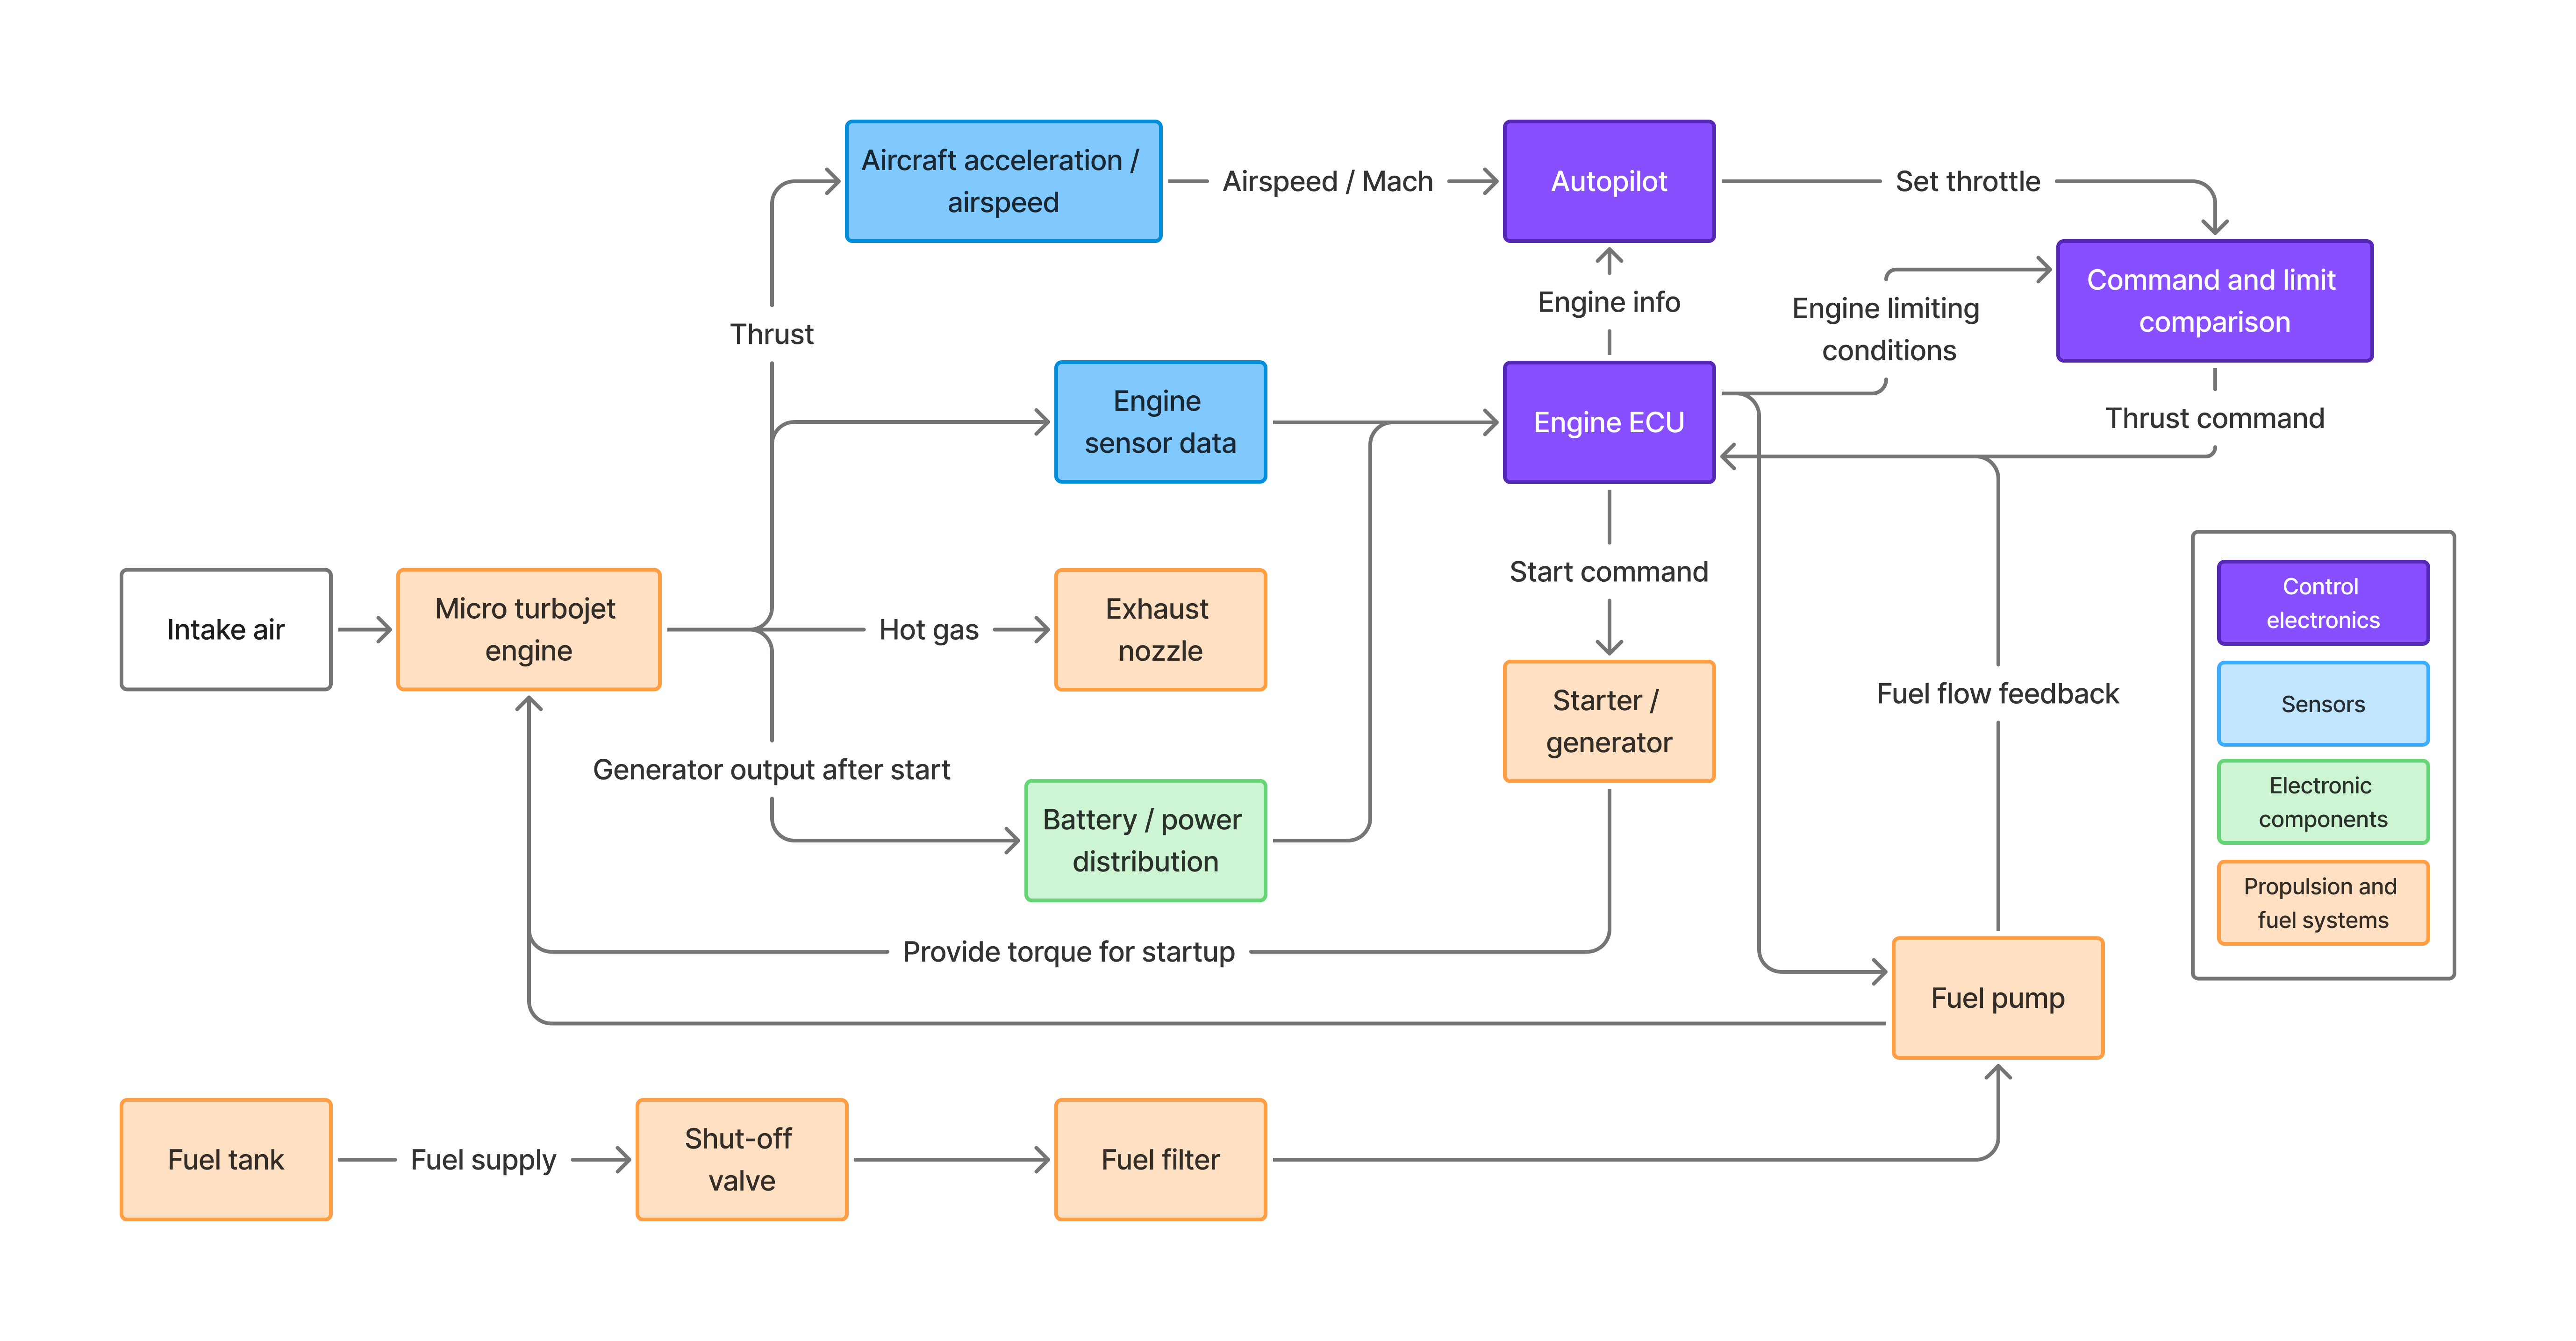
\includegraphics[width=\linewidth]{figures/HUGO propulsion system control feedback diagram.png}
    \caption{HUGO propulsion system diagram}
    \label{fig:prop_diagram}
\end{figure}
%\subsection{Payload systems}
% \label{subsec:payload_systems}

% HUGO will allow for extra payload to be mounted onboard, such as sensors and research equipment. By the mission requirements, the payload must have a cargo volume of at least 5 litres and support an additional weight of 5 kg. The cargo bay will be located close to the wing leading edge to minimize the impact on the dynamic stability of the aircraft. This choice was made since the engine and fuel will be aft of the trailing edge, affecting the longitudinal trim balance. A more detailed analysis of the internal payload mounting and contents will foloin the following step of the design.

%\textbf{Landing Gear Volume}

%The landing gear has been discussed in \autoref{sec:Landing_gear_config}, where its dimensions have been computed for each iteration. Following the trade-off process, it was decided to continue moving forward with design HUG-CFG-303, incorporating a retractable buried landing gear. Based on the analysis, the landing gear will have the dimensions mentioned in \autoref{tab:landing gear dimensions}. To estimate the space taken by the landing gear, its cuboid volume, with a 5 mm margin in every direction is computed. The volume occupied by each leg is 0.00057915 $m^3$, in total 0.0011583 $m^3$ of internal volume occupied by the undercarriage.
%\begin{table}[H]
%     \centering
%     \caption{Dimensions of the chosen landing gear}
%     \begin{tabular}{|c|c||c|c||c|c|}
%     \hline
%         \textbf{Dimension} & \textbf{Value [m]} & \textbf{Dimension} & \textbf{Value [m]} & \textbf{Dimension} & \textbf{Value [m]} \\
%         \hline \hline
%          Nose gear x poz & 0.272 & 
%          Fuselage gear x poz & 2.570 &
%          Fuselage gear y poz & 0.231 \\\hline 
%          Gear height & 0.167 & Wheel diameter & 0.085 & Strut and wheel width & 0.025\\\hline
         
%     \end{tabular}
    
%     \label{tab:landing gear dimensions}
% \end{table}


